\section{Overview}
\figref{fig:workflow} shows the main structure of the system. 
The user inputs some queries containing certain actions. Our system will
first detect whether it is an action concept triple, or a noun concept.
If it is an action concept triple, the system will find its noun abstractions
in the mapping we obtained offline, and expand the query with the noun 
abstractions. If it is a noun abstraction, then the system could just
search as it is because beforehand we would traverse the database
and convert action instances into noun abstractions so that news containing
them could be searched.

\begin{figure}[h!]
    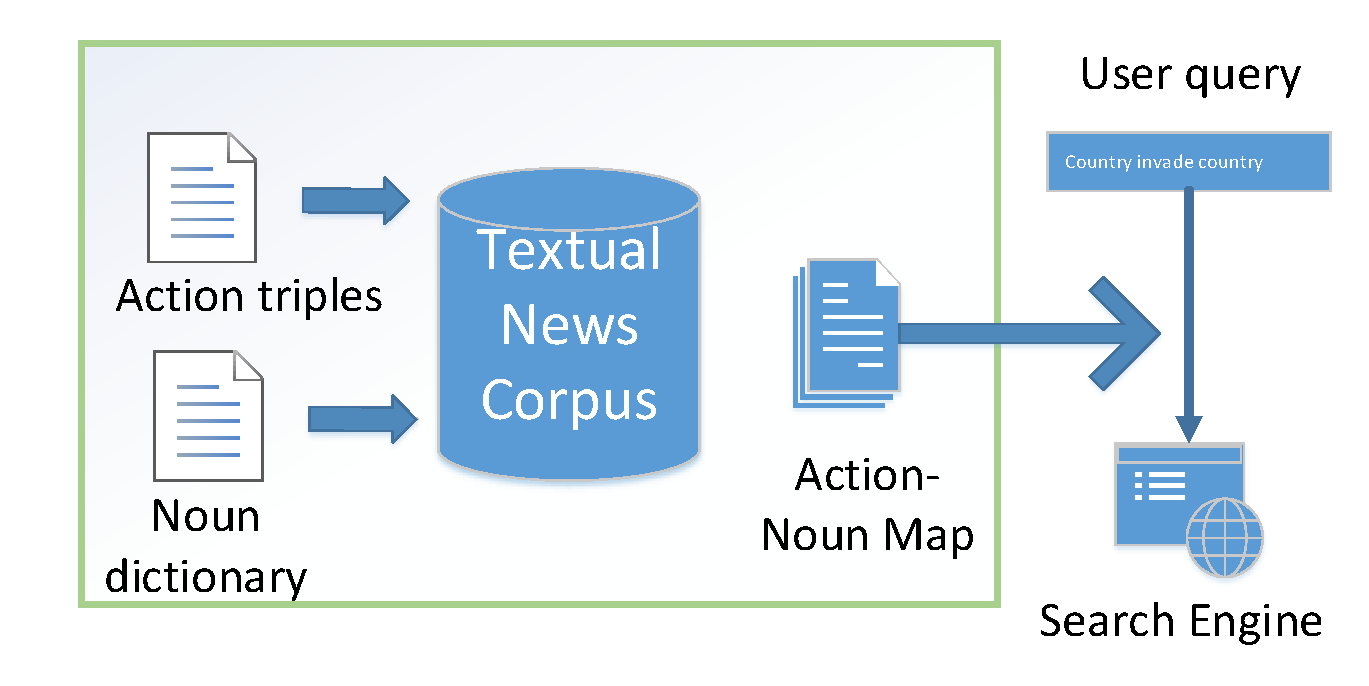
\includegraphics[width=0.95\linewidth]{img/ac1.pdf}
    \caption{workflow}
    \label{fig:workflow}
\end{figure}


The most important component in this project is to
abstract action triples by noun concepts. Here are some definitions we will use throughout
this paper:
\begin{itemize}
\item action concept: A triple consists of subject, predicate and object. Both subject and object are concepts in a predefined set.
    For example, ``country invade country'', ``company buy company'', ``person play instrument'', etc.
\item noun concept: An abstract noun that has multiple instances. 
    In this project we care about those nouns that could summarize an action.  
    For example, ``acquisition'', ``war'', ``performance'' etc.
\item action instance: A triple that is an instantiation of an action concept. Namely the subject and object are instances of the
    subject concept and object concept in action concept. For example, ``Germany invaded France'' would be an instance of ``country 
        invade country'', ``Google bought Deepmind'' would be an instance of ``company buy company''.
\end{itemize}
